\documentclass[a4paper,12pt]{article}

%%% Работа с русским языком
\usepackage{cmap}					% поиск в PDF
\usepackage{mathtext} 				% русские буквы в формулах
\usepackage[T2A]{fontenc}			% кодировка
\usepackage[utf8]{inputenc}			% кодировка исходного текста
\usepackage[english,russian]{babel}	% локализация и переносы

%%% Дополнительная работа с математикой
\usepackage{amsmath,amsfonts,amssymb,amsthm,mathtools} % AMS
\usepackage{icomma} % "Умная" запятая: $0,2$ --- число, $0, 2$ --- перечисление

%% Номера формул
%\mathtoolsset{showonlyrefs=true} % Показывать номера только у тех формул, на которые есть \eqref{} в тексте.
%\usepackage{leqno} % Нумерация формул слева

%% Свои команды
\DeclareMathOperator{\sgn}{\mathop{sgn}}

%% Перенос знаков в формулах (по Львовскому)
\newcommand*{\hm}[1]{#1\nobreak\discretionary{}
{\hbox{$\mathsurround=0pt #1$}}{}}

%%% Работа с картинками
\usepackage{graphicx}  % Для вставки рисунков
\graphicspath{{Materials/graphics/}{Materials/}}  % папки с картинками
\setlength\fboxsep{3pt} % Отступ рамки \fbox{} от рисунка
\setlength\fboxrule{1pt} % Толщина линий рамки \fbox{}
\usepackage{wrapfig} % Обтекание рисунков текстом

%%% Работа с таблицами
\usepackage{array,tabularx,tabulary,booktabs} % Дополнительная работа с таблицами
\usepackage{longtable}  % Длинные таблицы
\usepackage{multirow} % Слияние строк в таблице

%%% Теоремы
\theoremstyle{plain} % Это стиль по умолчанию, его можно не переопределять.
\newtheorem{theorem}{Теорема}[section]
\newtheorem{proposition}[theorem]{Утверждение}
 
\theoremstyle{definition} % "Определение"
\newtheorem{corollary}{Следствие}[theorem]
\newtheorem{problem}{Задача}[section]
 
\theoremstyle{remark} % "Примечание"
\newtheorem*{nonum}{Решение}

%%% Программирование
\usepackage{etoolbox} % логические операторы

%%% Страница
%\usepackage{extsizes} % Возможность сделать 14-й шрифт
\usepackage{geometry} % Простой способ задавать поля
	\geometry{top=25mm}
	\geometry{bottom=30mm}
	\geometry{left=25mm}
	\geometry{right=25mm}
 %

%%% Способ сделать тоже самое(но красивее:)
%\usepackage[margin=0.8in]{geometry}

 
\usepackage{fancyhdr} % Колонтитулы
 	\pagestyle{fancy}
 	\renewcommand{\headrulewidth}{0mm}  % Толщина линейки, отчеркивающей верхний колонтитул
 	\lfoot{}
 	\rfoot{}
 	\rhead{}
 	\chead{}
 	\lhead{ }
 	% \cfoot{Нижний в центре} % По умолчанию здесь номер страницы

\usepackage{setspace} % Интерлиньяж
%\onehalfspacing % Интерлиньяж 1.5
%\doublespacing % Интерлиньяж 2
%\singlespacing % Интерлиньяж 1

\usepackage{lastpage} % Узнать, сколько всего страниц в документе.

\usepackage{soulutf8} % Модификаторы начертания

\usepackage{hyperref}
\usepackage[usenames,dvipsnames,svgnames,table,rgb]{xcolor}
\hypersetup{				% Гиперссылки
    unicode=true,           % русские буквы в раздела PDF
    pdftitle={Заголовок},   % Заголовок
    pdfauthor={Автор},      % Автор
    pdfsubject={Тема},      % Тема
    pdfcreator={Создатель}, % Создатель
    pdfproducer={Производитель}, % Производитель
    pdfkeywords={keyword1} {key2} {key3}, % Ключевые слова
    colorlinks=true,       	% false: ссылки в рамках; true: цветные ссылки
    linkcolor=red,          % внутренние ссылки
    citecolor=green,        % на библиографию
    filecolor=magenta,      % на файлы
    urlcolor=cyan           % на URL
}

%\renewcommand{\familydefault}{\sfdefault} % Начертание шрифта

\usepackage{multicol} % Несколько колонок

% Мои "дополнительные" пакеты
\usepackage{textcase} 
\usepackage{pdfpages}
\usepackage{amsmath}
\usepackage{titlesec}
\usepackage{floatrow}
\usepackage{verbatim}
\usepackage{lipsum}

\author{Подкидышев Алексей}
\title{Студент МФТИ ФИВТ - 1ый курс}
\date{\today}

%% Делаем красивый header:
\fancyhead[RO]{\footnotesize{\scshape\nouppercase{~\leftmark}}}
%% Делаем красивый header END

%Делаем большой отступ между section и subsection
\titlespacing*{\section} {0pt}{3.5ex plus 1ex minus .2ex}{2.7ex plus .2ex}
\titlespacing*{\subsection} {0pt}{3ex plus 1.5ex minus .3ex}{1.7ex plus .2ex}

\begin{document}

\begin{titlepage}


\begin{center}
	\textit{\MakeTextUppercase{федеральное государственное автономное учреждение}}
		
	\vspace{0.5ex}
	
	\textbf{ \\ \MakeTextUppercase{<<Московский Физико-технический институт>>}}
\end{center}
\vspace{13ex}
\begin{flushright}
	\noindent
	{Подкидышев Алексей Сергеевич}
	\\
	\textit{Студент факультета инноваций\\ и высоких технологий\\(группа 790)}
\end{flushright}
\begin{center}
	\vspace{23ex}
	\line(1,0){350}\\[4ex]
	{\LARGE\textbf{Лабораторная работа 2.2.1}}
	\vspace{2ex}
	
		
	\textbf{\large{<<Исследование взаимной диффузии газов>>}}\\[3ex]
	\line(1,0){350}\\[5ex]
	\vfill
	Долгопрудный 
	
	{\today}
\end{center}

\end{titlepage}
\renewcommand{\headrulewidth}{0.7pt}

\section{Описание работы}
\subsection{Цель, оборудование}\
\noindent \textbf{Цель работы:} 

\begin{enumerate}

\item Регистрация  зависимости  концентрации   гелия в воздухе от времени с помощью датчиков теплопроводности при разных начальных давлениях смеси газов;
\item Определение коэффициента диффузии по результатам измерений.

\end{enumerate}

\noindent \textbf{В работе используются:} \\
\indent Измерительная установка; форвакуумный насос; баллон с газом (гелий); манометр; источник питания; магазин сопротивлений; гальванометр; секундомер.

\begin{figure}[H]
{\includegraphics[width=1\linewidth]{pic1.png}}\ 
\caption{Установка для исследования взаимной диффузии газов. Схема крана K6. Мостовая схема с датчиками теплопроводности для измерения разности концентраций газов.}

\end{figure}


\subsection{Теория}
\indent Рассмотрим процесс выравнивания концентрации. Закон Фика:
$$j=-D\frac{\partial n}{\partial x} \text{\hspace{3ex}	- \hspace{2ex}Плотность потока}$$
(Количество частиц, пересекающих единичную площадку в единицу времени)\\
В нашем случае ввиду того что, а) объем соединительной трубки мал по сравнению с объемами сосудов, б) концентрацию газов внутри каждого сосуда можно считать постоянной по всему объему.
$$J=-DS\frac{n_1-n_2}{l}$$
Изменение компонента в сосудах: $V_1\Delta n_1=-V_2\Delta n_2$\\
\ \\
С другой стороны $V_1\Delta n_1=J\Delta t$ и $V_1\frac{dn_1}{dt}=-DS\frac{n_1-n_2}{l}$; \ \ \  Аналогично $V_2\frac{dn_2}{dt}=DS\frac{n_1-n_2}{l}$\\
\ \\
Тогда $$\frac{d(n_1-n_2)}{dt}=-\frac{n_1-n_2}{l} \frac{V_1+V_2}{V_1V_2}$$
Проинтегрируем и получим, что
\begin{equation}
n_1-n_2=\Delta n=\Delta n_0 \cdot e^{-t/\tau} 
\end{equation}

\begin{equation}
 \tau=\frac{V_1V_2}{V_1+V_2}\frac{l}{SD} 
\end{equation}

%\begin{equation}
% V_1=V_2=V/=\frac{Vl}{2SD} 
%\end{equation}

 При заполнении сосудов смесями различного состава возникает «разбаланc» моста. При незначительном различии в составах смесей показания гальванометра, подсоединённого к диагонали моста, будут пропорциональны разности концентраций примеси. В процессе диффузии
разность концентраций убывает по экспоненте, и значит по тому же закону изменяются во времени показания гальванометра
$$U=U_0 \exp(-t/\tau)$$

 Для измерения концентраций в данной работе используется зависимость теплопроводности газовой смеси от ее состава. Количество тепла, передающееся от тонкой проволоки $R_\text{пр}$, протянутой вдоль оси цилиндра c радиусом $R_\text{ц}$ к его стенке равна: 

\begin{equation}
\underbrace{Q = \varkappa \cdot \dfrac{2\Pi L}{\ln{\dfrac{R_\text{ц}}{r_\text{пр}}}} \cdot (T_1 - T_2)}_{\text{где $\varkappa$ - теплопроводность; L - длина нити; T1, T2 - температура проволочки и стенки}}
\end{equation}

\newpage

\section{Ход работы}

\subsection{Подготовка установки для измерения}\
\indent Включим питание электрической схемы установки. Очистим установку от всех газов. Запустим воздух до рабочего давления $P_\text{раб}$. Сбалансируем мост. Заполним установку рабочей смесью и приступим к измерению: откроем соответствующие краны и снимем зависимость показания вольтметра от времени с помощью компьютера.

\begin{figure}[H]
\begin{floatrow}

{\includegraphics[width=0.4\linewidth]{comp.jpg}}
\hspace{5ex}

{\includegraphics[width=0.4\linewidth]{comp2.jpg}}

\caption{Интерфейс программы обрабатывающей показания вольтметра от времени}
\end{floatrow}

\end{figure}



\subsection{Измерения}

\begin{figure}[H]

\caption{40 и 80 торр соответственно}

\begin{tabular}{m{0.43\linewidth}m{0.43\linewidth}}

{\includegraphics[width=0.59\linewidth]{izm1.jpg}}
&
\begin{tabular}[r]{|l|l|l|}
\hline
t,c     & U, y.e  & ln(u/U\_0) \\ \hline
0,000   & 255,000 & 0,000      \\ \hline
12,950  & 249,000 & 0,024      \\ \hline
25,890  & 238,100 & 0,069      \\ \hline
38,840  & 229,200 & 0,107      \\ \hline
51,790  & 219,200 & 0,151      \\ \hline
64,740  & 212,700 & 0,181      \\ \hline
77,680  & 202,000 & 0,233      \\ \hline
90,630  & 194,000 & 0,273      \\ \hline
103,580 & 187,000 & 0,310      \\ \hline
116,530 & 180,000 & 0,348      \\ \hline
129,470 & 173,100 & 0,388      \\ \hline
142,420 & 168,000 & 0,417      \\ \hline
155,370 & 161,300 & 0,458      \\ \hline
168,320 & 154,000 & 0,504      \\ \hline
181,260 & 148,500 & 0,541      \\ \hline
194,210 & 144,000 & 0,571      \\ \hline
207,160 & 139,000 & 0,607      \\ \hline
220,110 & 134,900 & 0,637      \\ \hline
233,050 & 130,000 & 0,674      \\ \hline
246,000 & 126,000 & 0,705      \\ \hline

\end{tabular}
\end{tabular}
\end{figure}

	
\begin{figure}[H]
\begin{tabular}{m{0.49\linewidth}m{0.49\linewidth}}
	
\begin{flushleft}
\caption{120 торр и 160 торр соответственно}
\label{my-label}
\begin{tabular}{|l|l|l|}
\hline
t, с   & U, y/e & ln(u/U\_0) \\ \hline
0,00   & 255,00 & 0,00       \\ \hline
25,68  & 243,00 & 0,05       \\ \hline
51,36  & 228,60 & 0,05       \\ \hline
77,05  & 245,00 & 0,17       \\ \hline
102,73 & 202,00 & 0,23       \\ \hline
128,41 & 190,20 & 0,29       \\ \hline
154,09 & 18,90  & 0,35       \\ \hline
179,77 & 168,00 & 0,42       \\ \hline
205,45 & 158,50 & 0,48       \\ \hline
231,14 & 149,00 & 0,54       \\ \hline
256,82 & 141,20 & 0,59       \\ \hline
282,50 & 134,00 & 0,64       \\ \hline
308,18 & 125,00 & 0,71       \\ \hline
333,86 & 119,00 & 0,76       \\ \hline
359,55 & 113,00 & 0,81       \\ \hline
385,23 & 106,80 & 0,87       \\ \hline
410,91 & 101,00 & 0,93       \\ \hline
436,59 & 95,60  & 0,98       \\ \hline
462,27 & 90,00  & 1,04       \\ \hline
487,95 & 86,00  & 1,09       \\ \hline
513,64 & 82,00  & 1,14       \\ \hline
539,32 & 78,00  & 1,19       \\ \hline
565,00 & 75,00  & 1,22       \\ \hline
\end{tabular}
\end{flushleft}
&
\label{my-label}
\begin{tabular}{|l|l|l|}
\hline
t, c   & U, y.e & ln(U/U0) \\ \hline
0      & 255    & 0        \\ \hline
19,18  & 250    & 0,02     \\ \hline
38,36  & 243,6  & 0,046    \\ \hline
57,55  & 237    & 0,073    \\ \hline
76,73  & 230    & 0,103    \\ \hline
95,91  & 223,1  & 0,134    \\ \hline
115,09 & 217    & 0,161    \\ \hline
134,27 & 210    & 0,194    \\ \hline
153,45 & 204,5  & 0,22     \\ \hline
172,64 & 199    & 0,248    \\ \hline
191,82 & 193    & 0,279    \\ \hline
211    & 187    & 0,31     \\ \hline
230,18 & 182    & 0,337    \\ \hline
249,36 & 177    & 0,365    \\ \hline
268,55 & 170    & 0,394    \\ \hline
287,73 & 167    & 0,423    \\ \hline
306,91 & 162    & 0,454    \\ \hline
326,09 & 158    & 0,479    \\ \hline
345,27 & 153    & 0,511    \\ \hline
364,45 & 149    & 0,537    \\ \hline
383,64 & 14434  & 0,569    \\ \hline
402,82 & 140,2  & 0,598    \\ \hline
\end{tabular}
\end{tabular}

\end{figure}	

\subsection{Графики}

\begin{figure}[H]
{\includegraphics[width=0.6\linewidth]{graph5.jpg}}\ 
\caption{40 торр}
\end{figure}

\begin{figure}[H]
{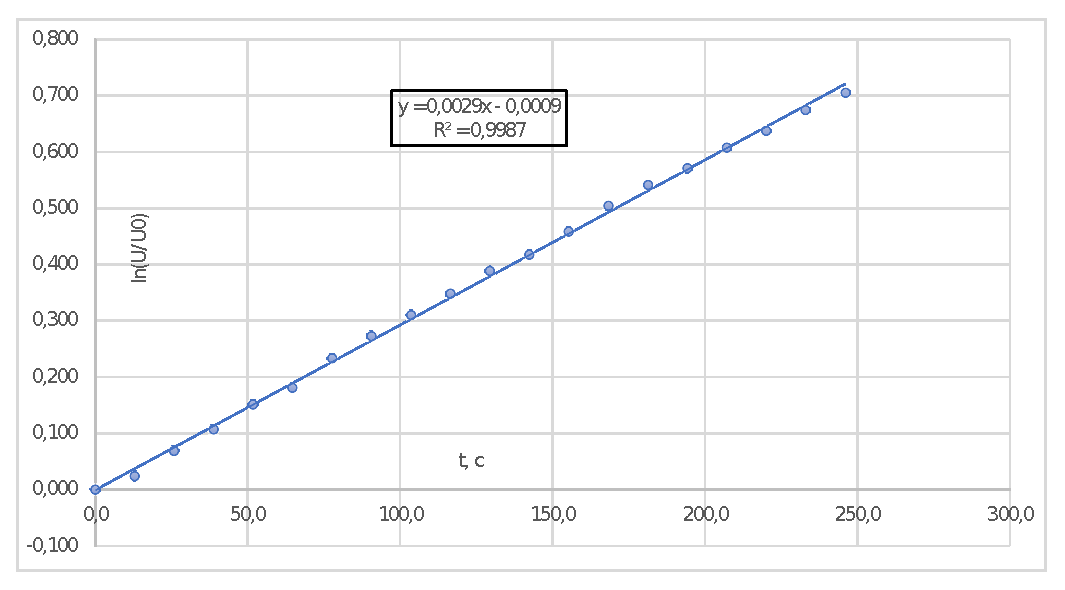
\includegraphics[width=0.7\linewidth]{graph2.eps}}\ 
\caption{80 торр}
\end{figure}

\begin{figure}[H]
{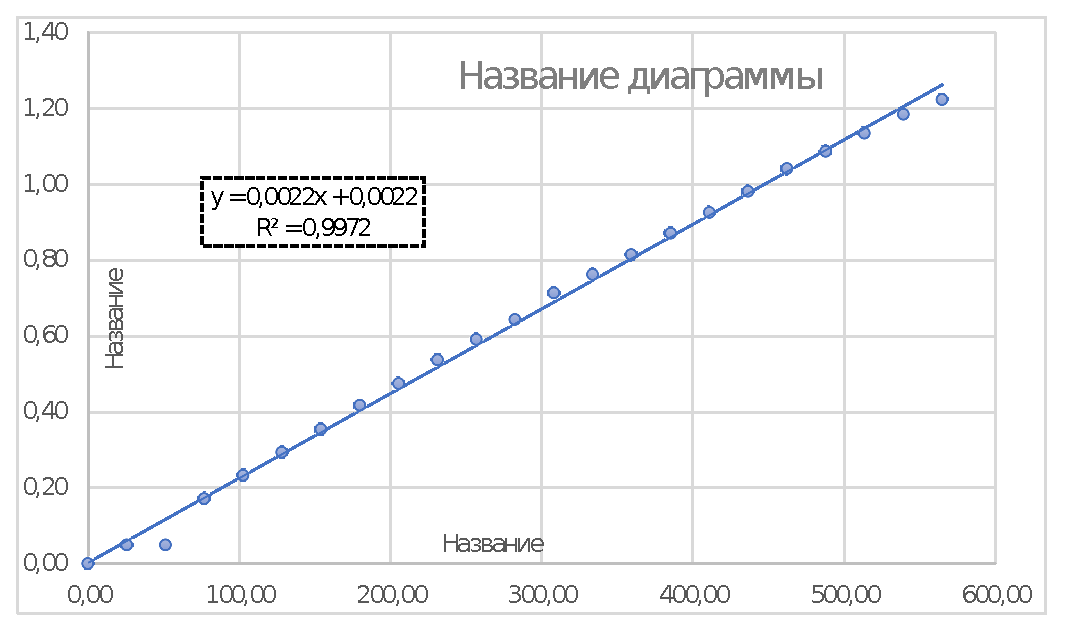
\includegraphics[width=0.7\linewidth]{graph3.eps}}\ 
\caption{120 торр}
\end{figure}

\begin{figure}[H]
{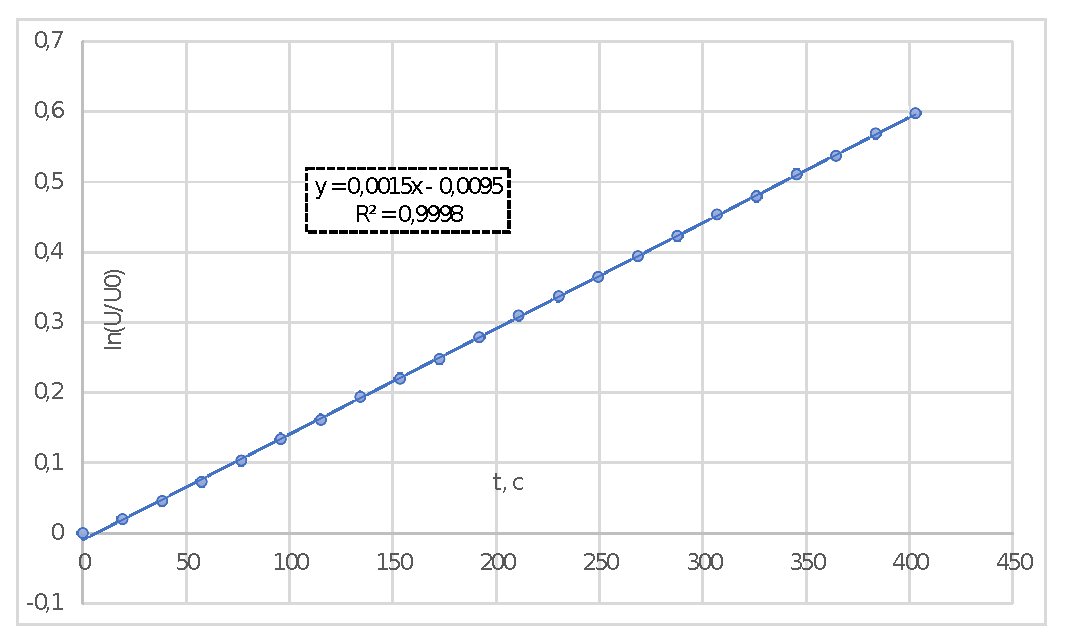
\includegraphics[width=0.7\linewidth]{graph4.eps}}\ 
\caption{160 торр}
\end{figure}

\subsection{Исследование полученных результатов}
Полученные данные:
\begin{table}[h!]
\centering
\caption{Коэффициенты взаимных диффузий для разных давлений}
\label{my-label}
\begin{tabular}{|l|l|l|l|l|}
\hline
$P_0$, торр                                              & 40       & 80       & 120      & 160      \\ \hline
1/P, $\text{торр}^{-1}$                               & 0,025    & 0,0125   & 0,008333 & 0,00625  \\ \hline
$\sigma_{1/p}$, $\text{торр}^{-1}$                     & 0,011979 & 0,000521 & 0,004688 & 0,006771 \\ \hline
a, $\text{c}^{-1}$                                & 2,18     & 2,9      & 2,2      & 1,5      \\ \hline
$\sigma_a$, $\text{c}^{-1}$                         & 0,015    & 0,705    & 0,005    & 0,695    \\ \hline
D, $10^{-3} \text{m}^2/c$        & 0,982    & 0,343    & 0,236    & 0,152    \\ \hline
$\sigma_d$, $10^{-3} \text{m}^{2}/c$ & 0,55375  & 0,08525  & 0,19225  & 0,27625  \\ \hline
\end{tabular}
\end{table}

Построим график зависимости коэффициента диффузии от обратного значения давления.

\begin{figure}[H]
{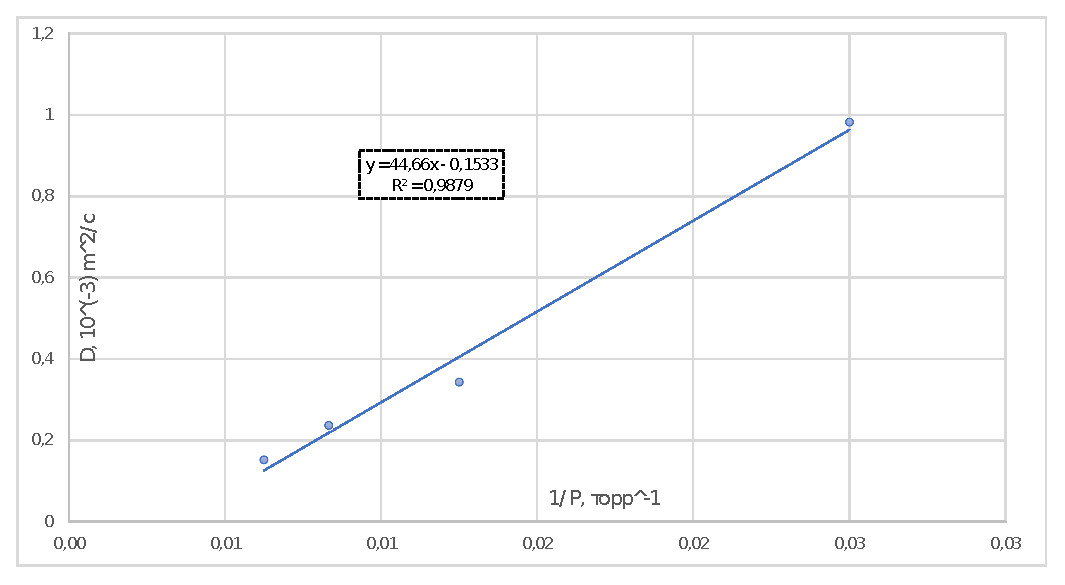
\includegraphics[width=0.7\linewidth]{finalGraph.eps}}\ 
\caption{График зависимости D(1/P)}
\end{figure}

\[\frac{dD}{d\Big(\dfrac{1}{P} \Big)} \equiv b\]

Аппроксимируя полученную зависимость, рассчитаем величину диффузии при атмосферном давлении и зная, что $b = (44 \pm 3) \text{торр m/c}$. Получаем:

\[D_\text{атм} = 0,55\  \dfrac{cm^2}{c} \]


\subsection{Погрешности}
\[\sigma_D = D \cdot \sqrt{\big( \dfrac{6V}{V} \big)^2 + \big(\dfrac{64S}{4S} \big)} \]\\
\[\mathcal{E}_D \approx 12.7 \%  \]

\section{Вывод}
\subsection{Длина свободного пробега, размер молекулы }

\begin{center}
\fbox{
$ D_\text{атм} = 0,55 \pm 0.08 \  \dfrac{cm^2}{c} $
}
\end{center}

Мы получили близкий к табличному значению результат($D_\text{табл}$ = 0,62 см2с), с небольшой погрешностью.

Оценим по полученным данным длину свободного давления $\lambda$ и размер молекулы:

\begin{center}
\fbox{
$ \lambda = 3D \cdot \sqrt{\dfrac{\mu}{3RT}} = (1.14 \pm 0.05) \cdot 10^{-7} \ m $
}
\end{center}


\begin{center}
\fbox{
$ \sqrt{\dfrac{kT}{P\lambda}} \simeq 10 ^{-10} \text{ m} $
}
\end{center}

Вывод: мы проверили требуемые зависимости и нашли $D_0$ = 0.55 см2/с коэффициент взаимной диффузии гелия и воздуха при нормальном атмосферном давлении и комнатной температуре.

\end{document}
